\subsection{VDP Implementation and Scalability}
\label{sec:lviz-imp}

There are two important challenges in implementing VDP in \code{lviz}.
Firstly, traces are usually much larger than the size of the screen.
The challenge is to be able to still have usable visualizations given that
there will not be sufficient pixels to show every event.
Secondly, rendering a VDP on large traces needs to be sufficiently fast to
meet interactive UI needs (i.e sub-second response).
Finally, our implementation takes advantage of parallelism given
the trend in multi-core processors.
In this section, we describe an effective and efficient implementation
which meets these challenges.

% Third, a ruler and barcode-like stripes for each axis of the DP
% are added to give additional insight about the region of the inner DP.
% as well as caching can help a lot in responsiveness.

% To fit $100K$ events in a small window screen, a pixel often has
% to accommodate more than one event which in turn will determine
% the brightness / intensity of the pixel.
% The intensity of a pixel is determined by how much
% events in that pixel is a match according to DP matching rule
% (ie. match by program name, path, etc...).
% The hash or message digest (ie. MD5) of the matched fields is
% used to speedup the process of matching tests.
% A pixel that has 10 matched events will look brighter than a pixel
% that has 3 matched events.
% This introduces a grayscale color extension to the DP.
% When the number of matched events are too big, sometimes it exceeds
% the threshold of a grayscale color range [0..255].
% To handle this case, we have $gamma$ normalization to adjust
% the brightness of the pixel. First, the intensity
% (the number of matched events) of each pixel is translated
% to a continuous range value between zero and one inclusive.
% Then each value is mapped to an equation $y = x^(1/g)$ where $g$ is the gamma value.
% The resulting value is then translated to a grayscale color range value [0..255].
% This allow us to reveal the low-intensity pixel.
% The difference can be seen in
% \TODO{Figure~\ref{xx} add explanation to the figures on the differences}.
% Another method to reveal the low intensity pixel is through
% histogram equalization \TODO{cite} which allows for areas with lower
% intensity to have a brighter display without affecting the global intensity.

\begin{figure}[tb]
\begin{center}
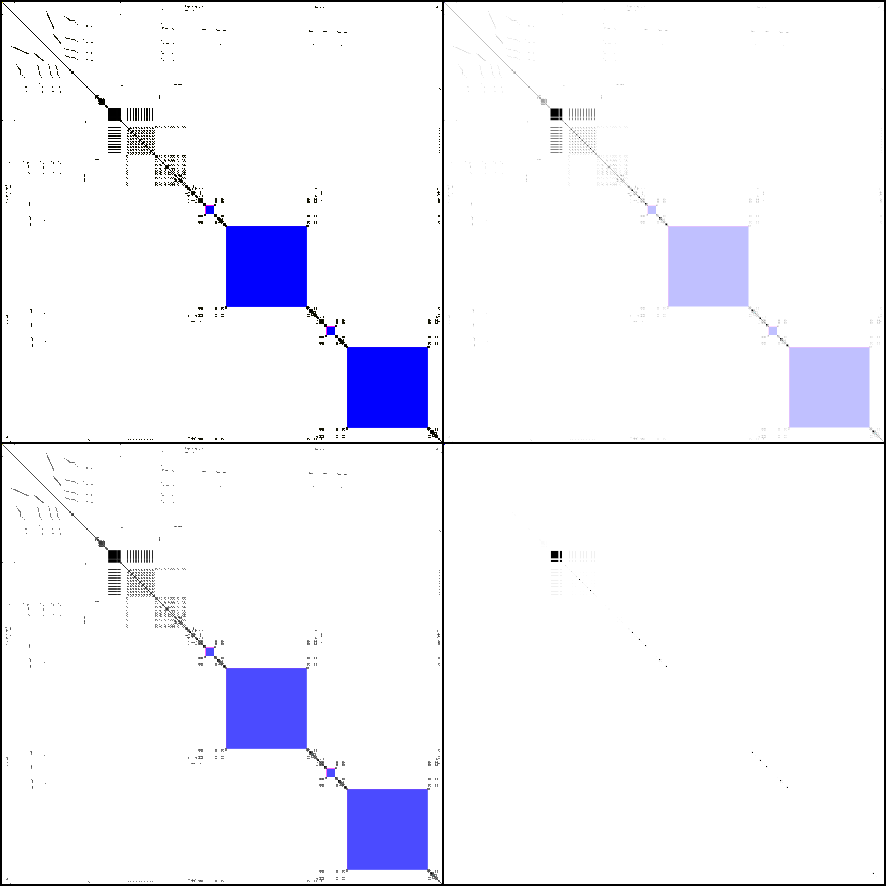
\includegraphics[width=0.5\textwidth]{lviz/gamma.png}
\caption{Clockwise from top-left:
histogram equalization, $\gamma=1$,
$\gamma=1/4$ and $\gamma=4$.
}
\label{fig:gamma}
\end{center}
\end{figure}

Consider a trace with $N$ events and
a display window size with width $W$ and height $H$.
For large traces, e.g. $N=10^6$, clearly $N \gg W$ and $N \gg H$,
and a binary DotPlot with two traces of $N=10^6$ corresponds to an
image with $10^{12}$ pixels (terrapixel).
Our VDP visualization aggregates multiple events into a single pixel,
normalizing it to RGB intensities between $0\ldots255$.
Unlike a digital photo, the intensity of a pixel could be up to $N$,
since aggregating events could end up with all of them
in a single pixel which could easily exceed 255.
\code{lviz} provides two options to deal with this issue by borrowing 
ideas from image processing.
The first is to simply normalize the values.
We extend normalization to include gamma correction, i.e. given an input value $x$,
the output value $y$ is mapped using the equation $y=x^{1/\gamma}$
(pure normalization corresponds to $\gamma = 1.0$).
The second option is histogram equalization which is
a well-known technique in image processing.

% \TODO{reviewer 3:
% The visual scalability discussion in section 4 opens up some serious questions.
% If I understand correctly, what is done is basically aggregation of colors like
% in image processing? This is very dangerous, since a visualization application
% should aggregate the actual data values, or more exactly even, the semantics of
% these values, and not the color mapped values. Just adding up or averaging
% colors can produce meaningless colors or even worse colors which exist in the
% used color map but have another meaning. See for example the work of D. Holten
% et al referred earlier or the work of T. Munzner on accordion drawing,
% guaranteed visibility, and the sequence juxtaposer comparison (available at
% http://www.cs.ubc.ca/~tmm/papers.html)
% }

Fig.~\ref{fig:gamma} shows our {\tt xcopy} example visualized
with various normalization options.
In this example with an event-ordered VDP,
the intensity of a pixel shows how many matching events there are in the DP.
We see that histogram equalization (the default) is usually effective
in allowing matching burst events (high intensity) to seen together
with spread out events (low intensity).
While smaller $\gamma$ shows details of the high intensity events,
larger $\gamma$ shows low intensity events.

Most of the cost of rendering a VDP has to do with various forms of
matching: applying DP matching, DP coloring and barcode rules.
We can optimize the rendering to reduce matching costs by pre-processing
the traces. \code{lviz} performs the pre-processing steps when reading the
traces. Subsequent visualizations such as zooming in then make use of
the pre-computed results of the pre-processing phase.

An event in the raw trace is simply a string.
The pre-processing steps involves reducing an event to
a digest value as a more compact representation for DP matching
to operate on and also pre-computing the
results of various coloring rules.
Each event is represented as a hash value which we call a {\em digest}.
The digest helps to speed up event comparisons
as comparing digest values of events is much faster than
the corresponding string comparison, e.g. string matching is slow
as the strings of an event property often have a long common prefix such
as absolute pathname.
The digest of an event is computed based on the DP matching rule that specifies
how to tell if events are considered similar (see Sec. ~\ref{sec:lviz-vis}).
For example, if the matching rule is 
{\em program name + operation type + resource name}, the digest
of the event is a hash on those three properties of the event in that order.
We will refer to all the events having the same digest under
the set of DP matching rules as a {\em digest group}.
Thus, the number of digest groups in a trace is equal to the number of distinct hash values.
Note that an event can only belong to one digest group and the hash function
should be good enough to be effectively collision free so that 
two events which do not match (according to the DP matching rule) are
not hashed to the same digest group.

% The DP coloring rules extend the visualization to 24-bit color DP.
% We employ a pre-processing strategy 
% to speedup the matching of color rules (DP and Barcode).
% Once two events are considered a match by the DP matching rule, 
% those events will be colored based on the DP color rules.
It is common that the pattern in a coloring rule only needs a string
match.
Since there can be many color rules, we want to avoid applying
to the matching events one rule at a time.
We instead employ the Aho-Corasick's string matching algorithm \cite{aho1975efficient}
to compile all the rules (the string patterns) into a single automaton.
This allows us to identify the color in a single pass
rather than multiple passes for each rule.

\begin{algorithm}[htb]
\KwIn{$L_X[0\ldots N-1]$ as log X; and $L_Y[0\ldots N-1]$ as log Y}
\KwOut{2D array $S[0\ldots W-1,0\ldots H-1]$ as pixel intensity}
\BlankLine
zero fill $S$\;
\For{$x\leftarrow 0$ \KwTo $N-1$}{
  \For{$y\leftarrow 0$ \KwTo $N-1$}{
    \If{$LX[x]=XY[y]$}{
      $S[xW/N,yH/N] ++$
    }
  }
}
\caption{Naive $O(N^2)$ Algorithm}
\label{alg:lviz-naive}
\end{algorithm}

The two pre-processing steps above are performed once and
cached in memory for later use when rendering the VDP.
The VDP rendering has to be fast as it is
used interactively for real-time browsing 
which entails zooming in on a region within the DP.
As the number of events in a trace, $N$, grows in order of hundreds of thousands,
the naive DP Algorithm~\ref{alg:lviz-naive}
takes $O(N^2)$ becomes infeasible.
To simplify our illustration, we assume both logs have the same number
of events.
We developed a new DP rendering algorithm which scales well to large traces.

\begin{algorithm}[htb]
\KwIn{$L_X[0\ldots N-1]$ as log X; and $L_Y[0\ldots N-1]$ as log Y}
\KwOut{Associative array $D_X[d]$ whose key $d$ is the digest of an event
and value is a set of integers representing indexes of events in $L_X$ whose
digests are $d$. Similarly for $D_Y[d]$.}
\BlankLine
\For{$x\leftarrow 0$ \KwTo $N-1$}{
  $d\leftarrow digest(L_X[x])$\;
  insert x to the set $D_X[d]$
}
\For{$y\leftarrow 0$ \KwTo $N-1$}{
  $d\leftarrow digest(L_Y[y])$\;
  insert y to the set $D_Y[d]$
}
\caption{Preprocessing step to get digest group}
\label{alg:lviz-algpre}
\end{algorithm}

\begin{algorithm}[htb]
\KwIn{$D_X[d]$ and $D_Y[d]$ from Algorithm~\ref{alg:lviz-algpre}}
\KwOut{2D array $S[0\ldots W-1,0\ldots H-1]$ as pixel intensity}
\BlankLine
zero fill $S$\;
\ForEach{digist $d$}{
  \ForEach{$x$ in $D_X[d]$}{
    \ForEach{$y$ in $D_Y[d]$}{
      $S[xW/N,yH/N] ++$
    }
  }
}
\caption{New Algorithm A}
\label{alg:lviz-alg1}
\end{algorithm}

The core of new DP rendering algorithm is based on two observations.
The first observation is that for each matching event,
a certain intensity value can be added incrementally.
Two events are considered a match if they are in the same digest group.
Events in different digest groups will never match thus will never be rendered.
The incremental algorithm effectively processes only the events
that contribute to the visualization and prunes all other events.
Consider digest group $D_i$ which has $S_i$ events.
It can be processed in time $O(S_i^2)$
and the result for this digest group can be added incrementally to the 
end result.
This significantly reduces the number of matching comparisons needed
from $O(N^2)$ down to $\sum_{i=1}^{G} S_i^2$
where $G$ is the number of digest groups in the trace.
Algorithm~\ref{alg:lviz-algpre} pre-process the two logs $L_X$ and $L_Y$
into digest groups stored in associative arrays $D_X$ and $D_Y$.
This preprocessing step takes $O(N)$ time and is executed only once.
Algorithm~\ref{alg:lviz-alg1} iterates each digest group and accumulates
the number of matches.

\begin{algorithm}[htb]
\KwIn{$D_X[d]$ and $D_Y[d]$ from Algorithm~\ref{alg:lviz-algpre}}
\KwOut{2D array $S[0\ldots W-1,0\ldots H-1]$ as pixel intensity}
\BlankLine
zero fill $S$\;
\ForEach{digist $d$}{
  declare temporary integer array $S_X[0\ldots W-1]$ and $S_Y[0\ldots H-1]$\;
  zero fill $S_X$ and $S_Y$\;
  \lForEach{$x$ in $D_X[d]$}{
    $S_X[xW/N] ++$
  }\;
  \lForEach{$y$ in $D_Y[d]$}{
    $S_Y[yH/N] ++$
  }\;
  \For{$x\leftarrow 0$ \KwTo $W-1$}{
    \For{$y\leftarrow 0$ \KwTo $H-1$}{
      $S[x,y]\leftarrow S[x,y]+S_X[x]\times S_Y[y]$
    }
  }
}
\caption{New Algorithm B}
\label{alg:lviz-alg2}
\end{algorithm}

However, in the worst case, a digest group $S_i$ can be as large as $N$.
This drawback leads us to the second observation which
gives an optimization for the case when the digest group size is large.
It exploits the fact that $N > W\times H$ and often also $N \gg W\times H$.
Consider a digest group with $S_i$ events.
The intensity (color) for each event in that group can be recorded as
its projection on the X and Y axis of the window.
This is easily done by keeping track of the color intensities in
two arrays with size $W$ and $H$ respectively in $O(S_i)$ time.
Therefore, the resulting DP on a window of size $W \times H$
can be drawn based on the projected intensities in $O(S_i + W\times H)$ time,
as shown in Algorithm~\ref{alg:lviz-alg2}.

\begin{algorithm}[htb]
\KwIn{$D_X[d]$ and $D_Y[d]$ from Algorithm~\ref{alg:lviz-algpre}}
\KwOut{2D array $S[0\ldots W-1,0\ldots H-1]$ as pixel intensity}
\BlankLine
zero fill $S$\;
\ForEach{digist $d$}{
  \nlset{$\alpha$} \uIf{$D_X[d]\times D_Y[d]<D_X[d]+D_Y[d]+W\times H$}{
    \ForEach{$x$ in $D_X[d]$}{
      \ForEach{$y$ in $D_Y[d]$}{
        $S[xW/N,yH/N] ++$
      }
    }
  } \Else{
    declare temporary integer array $S_X[0\ldots W-1]$ and $S_Y[0\ldots H-1]$\;
    zero fill $S_X$ and $S_Y$\;
    \lForEach{$x$ in $D_X[d]$}{
      $S_X[xW/N] ++$
    }\;
    \lForEach{$y$ in $D_Y[d]$}{
      $S_Y[yH/N] ++$
    }\;
    \For{$x\leftarrow 0$ \KwTo $W-1$}{
      \For{$y\leftarrow 0$ \KwTo $H-1$}{
        $S[x,y]\leftarrow S[x,y]+S_X[x]\times S_Y[y]$
      }
    }
  }
}
\caption{Combined algorithm.
(Line $\alpha$ can be further tuned with some constant factors)}
\label{alg:lviz-alg3}
\end{algorithm}

Both algorithms can be combined together to
get the best of both worlds, which gives
a DP rendering time complexity of $\sum_{i=1}^{G} min(S_i^2, S_i + W H)$,
as shown in Algorithm~\ref{alg:lviz-alg3}.
That is, for each digest group $S_i$ that satisfies $S_i^2 < S_i+W H$, 
the $O(S_i^2)$ algorithm is used;
otherwise, the $O(S_i + W H)$ algorithm is used to obtain a sub-image.
Adding the intensities of all the sub-images of all digest groups gives the final image.

We illustrate the complexity of the algorithm to process $N=10^6$ events.
The worst case is when the number of digest groups $G$ is $10^3$
and each digest group has size $10^3$.
Suppose the window screen size is $1000\times 1000$.
Then the first $O(S^2)$ algorithm is used giving $GS^2 = 10^9$ operations.
If the window size is resized to $600\times 400$, then
the second $O(S+W H)$ algorithm is used giving $G(S+WH)=2.41\times 10^8$ operations.
This is much faster than the naive algorithm which would take $O(10^{12})$
operations.
The best case is achieved when each digest group only contains one event.
This means $G = 10^6$ and the number of operations
is $G S^2=10^6$.
Another good case is when there is only one digest group,
so $S=10^6$ and the number of operations is $G(S + WH)=1.24\times10^6$.

\code{lviz} is multi-threaded to make use of multi-core processors.
The pre-processing steps and rendering algorithms can be easily parallelized.
The events in the trace can be split up into several sub-traces and 
the pre-processing can be applied to each sub-trace
independently and in parallel.
We implemented and tested the rendering algorithm using
OpenJDK 1.6.0\_18 (64bit) on an Intel Core i7-960 3.20GHz
machine with 12G RAM.
An uncompressed 120MB trace file with 558K events took 2.8 seconds
to read and finish the two pre-processing steps using 8 threads.
To see the effectiveness of parallel pre-processing, it took 6.0 seconds,
when the execution is single-threaded.
In our rendering algorithm, each digest group can be processed
independently and in parallel as there is no dependency between digest groups.
We also render all the sub-components
of a VDP, the DP, barcodes, and histograms in parallel.
It took about 0.5 seconds to render the trace where the DP has 550K events
on both axis.
Thus, \code{lviz} can process large traces with sufficient real-time response
when the user interactively zooms/resizes the VDP or changes the histogram.

To speed up subsequent runs, \code{lviz} creates a cache containing the results
of the pre-computations of the digest, DP color, barcodes color
of each event since they require the most computation
and are the bottleneck of the system. The cache avoids recalculating the
digest and the coloring rules every time the program is run.
This cache is rebuilt if the corresponding rules change.
Loading from the cache skips the pre-computation steps and
cuts down the trace loading time to 1.3 seconds.
The speedup is more significant when the matching and coloring rules are
more complicated.

% \TODO{reviewer 2:
% The scalability solution seems, from what I can read, well thought. However I
% wonder if a comparatively fast result, if not a faster one, could not have been
% obtained, with less programming effort, by using a pixel shaders or CUDA
% implementation.
% }

% While the DP treats each event independently,
% RTG has to show the connections
% between events for visualizing the resource life cycle.
% If we consider each event as an operation on a resource
% (e.g. file or registry key),
% each resource is associated with a sequence of operations which includes
% creating a new one, opening an existing one, reading, writing/modifying, closing, deletion.
% If we further assume the resource life cycle has three states:
% non-existence, exists but not
% opened, opened, we can use the sequence of operations to
% reconstruct the state transitions for RTG visualization.
% However, there are some exceptions to be noted.
% Firstly, we may be dealing with a trace
% only during some time period, i.e. some
% resource can be opened before logging happens,
% thus we have to ``guess'' the initial state of the resource.
% We employ a heuristic based on the first observed operation of each resource.
% Secondly, file deletion in Windows is done in a special system call
% {\tt NtSetInformationFile} which puts file into ``delete after close'' state.
% In order to delete a file, one should first open the file,
% then call {\tt NtSetInformationFile} to set the ``delete after close'' state,
% finally close the file and if no other processes are opening the file, it will
% be deleted.
% Lastly, there is an additional rename operation
% which is translated in our RTG as a combination
% of deletion and creation operations.
